\documentclass[12pt,a4paper]{article}
\usepackage[utf8]{inputenc}
\usepackage[T1]{fontenc}
\usepackage{amsmath}
\usepackage{amsfonts}
\usepackage{amssymb}
\usepackage{graphicx}
\usepackage{geometry}
\usepackage{float}
\usepackage{fancyhdr}
\usepackage{lastpage}
\usepackage[unicode=true]{hyperref}
\usepackage{booktabs}
\usepackage{textcomp}
\usepackage[english]{babel}
\usepackage{pifont}
\usepackage{gensymb}  % For \degree symbol
\usepackage{caption}  % For better caption handling

% Configure hyperref
\hypersetup{
    unicode=true,
    pdftitle={Civil Engineering Project - Dataset 5},
    pdfauthor={Warsaw University of Technology},
    pdfsubject={Structural and Thermal Analysis},
    pdfkeywords={civil engineering, structural analysis, thermal analysis},
    bookmarksnumbered=true,
    bookmarksopen=true,
    bookmarksopenlevel=1,
    colorlinks=true,
    linkcolor=blue,
    citecolor=blue,
    urlcolor=blue,
    pdfstartview={FitH},
    pdfpagemode={UseOutlines}
}

% No need to define degree symbols - using gensymb package

\geometry{
    a4paper,
    total={170mm,257mm},
    left=20mm,
    top=22.5mm,
    headheight=14.5pt
}

\pagestyle{fancy}
\fancyhf{}
\rhead{Dataset 5 Analysis}
\lhead{Civil Engineering Project}
\rfoot{Page \thepage\ of \pageref{LastPage}}

\begin{document}

\title{Civil Engineering Project - Dataset 5\\
Structural and Thermal Analysis Report}
\author{Warsaw University of Technology\\
Environmental Engineering Department}
\date{\today}

\maketitle
\thispagestyle{fancy}

\section{Building Specifications}
\subsection{Geometric Parameters}
\begin{itemize}
    \item Width (b) = 7.2 m
    \item Length 1 (L1) = 6.6 m
    \item Length 2 (L2) = 10.8 m
    \item Height 1 (h1) = 2.5 m
    \item Height 2 (h2) = 2.65 m
    \item Roof angle ($\alpha$) = 16\degree
    \item Purlin spacing (s) = 1.1 m
    \item Ground Level = -1.4 m.a.s.l
\end{itemize}

\subsection{Materials}
\begin{itemize}
    \item Walls: MAX 220 block
    \item Thermal insulation: Mineral wool
    \item Roofing: Steel tile 0.6 mm
    \item Structure: C27 timber class
\end{itemize}

\section{Structural Analysis}

\subsection{A. Rafter Analysis}
\subsubsection{Material Properties - C27 Timber}
According to EN 338, the C27 timber class has the following characteristic properties:

\begin{equation}
\begin{aligned}
f_{m,k} &= 27 \text{ N/mm}^2 & \text{(characteristic bending strength)} \\
f_{c,0,k} &= 22 \text{ N/mm}^2 & \text{(characteristic compression strength)} \\
E_{0,mean} &= 11.5 \text{ kN/mm}^2 & \text{(mean modulus of elasticity)} \\
\rho_k &= 370 \text{ kg/m}^3 & \text{(characteristic density)}
\end{aligned}
\end{equation}

\noindent
Design factors according to EN 1995-1-1:
\begin{itemize}
    \item $\gamma_M$ = 1.3 (partial safety factor for timber)
    \item $k_{mod}$ = 0.8 (modification factor for Service Class 2)
\end{itemize}

\subsubsection{Design Strength Calculations}
The design bending strength is calculated as:
\begin{equation}
f_{m,d} = \frac{k_{mod} \times f_{m,k}}{\gamma_M} = \frac{0.8 \times 27}{1.3} = 16.62 \text{ N/mm}^2
\end{equation}

\noindent
\textit{where:}
\begin{itemize}
    \item $f_{m,d}$ is the design bending strength
    \item $k_{mod}$ accounts for load duration and moisture content
    \item $f_{m,k}$ is the characteristic bending strength
    \item $\gamma_M$ is the partial safety factor for material properties
\end{itemize}

\subsubsection{Load Analysis}
According to Eurocode (EN 1990, EN 1991), we must consider all relevant actions on the structure:

\paragraph{Dead Loads (G)}
The permanent actions include:
\begin{equation}
\begin{aligned}
g_{k,tile} &= 0.047 \text{ kN/m²} & \text{(steel tile 0.6mm)} \\
g_{k,struct} &= 0.15 \text{ kN/m²} & \text{(supporting structure)} \\
g_{k,total} &= 0.197 \text{ kN/m²} & \text{(total dead load)}
\end{aligned}
\end{equation}

\paragraph{Snow Load (S)}
According to EN 1991-1-3 (Eurocode 1: Actions on structures - Part 1-3: General actions - Snow loads), the characteristic snow load on the roof is calculated using the following formula:
\begin{equation}
s = \mu_1 \times C_e \times C_t \times s_k \quad [\text{kN/m²}]
\end{equation}

\noindent
\textit{where:}
\begin{itemize}
    \item $s$ is the snow load on the roof [kN/m²]
    \item $\mu_1$ is the roof shape coefficient, determined by roof pitch angle:
        \begin{itemize}
            \item For $\alpha = 16\degree$: $\mu_1 = 0.8$ (linear interpolation between 0.8 for $\alpha \leq 30\degree$ and 0.0 for $\alpha \geq 60\degree$)
        \end{itemize}
    \item $C_e$ is the exposure coefficient:
        \begin{itemize}
            \item $C_e = 1.0$ for normal topography (no significant removal of snow by wind)
        \end{itemize}
    \item $C_t$ is the thermal coefficient:
        \begin{itemize}
            \item $C_t = 1.0$ for normal thermal insulation ($< 1.0$ only for glazed roofs)
        \end{itemize}
    \item $s_k = 0.7 \text{ kN/m²}$ is the characteristic ground snow load for Warsaw region (Zone 2)
\end{itemize}

\noindent
Step-by-step calculation:
\begin{enumerate}
    \item Determine $\mu_1$ based on roof angle:
        \begin{itemize}
            \item $\alpha = 16\degree \rightarrow \mu_1 = 0.8$
        \end{itemize}
    \item Verify exposure conditions:
        \begin{itemize}
            \item Normal topography $\rightarrow C_e = 1.0$
        \end{itemize}
    \item Check thermal conditions:
        \begin{itemize}
            \item Standard roof insulation $\rightarrow C_t = 1.0$
        \end{itemize}
    \item Look up ground snow load:
        \begin{itemize}
            \item Warsaw (Zone 2) $\rightarrow s_k = 0.7 \text{ kN/m²}$
        \end{itemize}
    \item Calculate roof snow load:
        \begin{equation}
        s = 0.8 \times 1.0 \times 1.0 \times 0.7 = 0.56 \text{ kN/m²}
        \end{equation}
\end{enumerate}

\paragraph{Wind Load (W)}
According to EN 1991-1-4 (Eurocode 1: Actions on structures - Part 1-4: General actions - Wind actions), the peak velocity pressure is calculated through a series of steps:

\subparagraph{1. Basic Wind Velocity}
The basic wind velocity is defined as:
\begin{equation}
v_b = c_{dir} \times c_{season} \times v_{b,0} \quad [\text{m/s}]
\end{equation}

\noindent
\textit{where:}
\begin{itemize}
    \item $v_b$ is the basic wind velocity [m/s]
    \item $c_{dir} = 1.0$ is the directional factor (recommended value)
    \item $c_{season} = 1.0$ is the season factor (recommended value)
    \item $v_{b,0} = 22 \text{ m/s}$ is the fundamental basic wind velocity for Warsaw region
\end{itemize}

\subparagraph{2. Mean Wind Velocity}
The mean wind velocity at height z is calculated as:
\begin{equation}
v_m(z) = c_r(z) \times c_o(z) \times v_b \quad [\text{m/s}]
\end{equation}

\noindent
\textit{where:}
\begin{itemize}
    \item $c_r(z)$ is the roughness factor
    \item $c_o(z) = 1.0$ is the orography factor (for flat terrain)
    \item For terrain category III (suburban area):
        \begin{itemize}
            \item $z_0 = 0.3 \text{ m}$ (roughness length)
            \item $z_{min} = 5 \text{ m}$ (minimum height)
        \end{itemize}
\end{itemize}

\subparagraph{3. Peak Velocity Pressure}
The peak velocity pressure at height z is given by:
\begin{equation}
q_p(z) = c_e(z) \times q_b = c_e(z) \times \frac{1}{2} \rho v_{b}^2 \quad [\text{kN/m²}]
\end{equation}

\noindent
\textit{where:}
\begin{itemize}
    \item $q_p(z)$ is the peak velocity pressure [kN/m²]
    \item $c_e(z) = 1.6$ is the exposure factor at height z = 2.65m
    \item $\rho = 1.25 \text{ kg/m³}$ is the air density
    \item $q_b$ is the basic velocity pressure [kN/m²]
\end{itemize}

\noindent
Step-by-step calculation:
\begin{enumerate}
    \item Calculate basic wind velocity:
        \begin{equation}
        v_b = 1.0 \times 1.0 \times 22 = 22 \text{ m/s}
        \end{equation}
    
    \item Calculate basic velocity pressure:
        \begin{equation}
        q_b = \frac{1}{2} \times 1.25 \times 22^2 = 0.302 \text{ kN/m²}
        \end{equation}
    
    \item Determine exposure factor:
        \begin{itemize}
            \item For z = 2.65m, terrain category III: $c_e(z) = 1.6$
        \end{itemize}
    
    \item Calculate peak velocity pressure:
        \begin{equation}
        q_p(z) = 1.6 \times 0.302 = 0.483 \text{ kN/m²}
        \end{equation}
\end{enumerate}

This peak velocity pressure is used for determining the wind forces on the building structure, considering pressure coefficients for different building surfaces.

\subsubsection{Ultimate Limit State Analysis}
According to EN 1990, we analyze two load combinations to determine the critical design load:

\paragraph{Load Combinations}
\begin{equation}
\begin{aligned}
E_{d1} &= 1.35G + 1.5S + 1.5\psi_0W \\
E_{d2} &= 1.35G + 1.5W + 1.5\psi_0S
\end{aligned}
\end{equation}

\noindent
\textit{where:}
\begin{itemize}
    \item $G$ = 0.25 kN/m² (total dead load)
    \item $S$ = 0.56 kN/m² (snow load)
    \item $W$ = 0.483 kN/m² (wind load)
    \item $\psi_0$ = 0.6 (combination factor)
\end{itemize}

Resulting in:
\begin{equation}
\begin{aligned}
E_{d1} &= 1.35(0.25) + 1.5(0.56) + 1.5(0.6)(0.483) = 1.401 \text{ kN/m²} \\
E_{d2} &= 1.35(0.25) + 1.5(0.483) + 1.5(0.5)(0.56) = 1.337 \text{ kN/m²}
\end{aligned}
\end{equation}

Design load: $E_d = \max(E_{d1}, E_{d2}) = 1.401 \text{ kN/m²}$

\subsection{B. Purlin Analysis (80×160mm)}
\subsubsection{Section Properties}
The purlin's geometric characteristics:
\begin{equation}
\begin{aligned}
A &= b \times h = 80 \times 160 = 12,800 \text{ mm}^2 \\
W &= \frac{b \times h^2}{6} = \frac{80 \times 160^2}{6} = 341,333 \text{ mm}^3 \\
I &= \frac{b \times h^3}{12} = \frac{80 \times 160^3}{12} = 27,306,667 \text{ mm}^4
\end{aligned}
\end{equation}

\subsubsection{Bending Moment Analysis}
Design load per purlin:
\begin{equation}
w = E_d \times s = 1.401 \times 1.1 = 1.541 \text{ kN/m}
\end{equation}

Maximum bending moment (simple beam):
\begin{equation}
M_{max} = \frac{w \times L^2}{8} = \frac{1.541 \times 1.8^2}{8} = 0.623 \text{ kNm}
\end{equation}

\subsubsection{Stress Verification}
Bending stress calculation:
\begin{equation}
\sigma_{m,d} = \frac{M_{max}}{W} = \frac{0.623 \times 10^6}{341,333} = 1.83 \text{ N/mm²}
\end{equation}

Verification against design strength:
\begin{equation}
\sigma_{m,d} = 1.83 \text{ N/mm²} < f_{m,d} = 16.62 \text{ N/mm²} \quad \checkmark
\end{equation}

\subsection{C. Column and Brace Analysis}
\subsubsection{Angle Brace Design (60×100mm)}
Force analysis for $45\degree$ brace:
\begin{equation}
N = E_d \times A_{trib} \times \sin(45\degree) = 1.401 \times 2.75 \times 0.707 = 2.71 \text{ kN}
\end{equation}

\noindent
\textit{where $A_{trib}$ is the tributary area = 1.1m × 2.5m = 2.75 m²}

Tensile stress verification:
\begin{equation}
\sigma_{t,0,d} = \frac{N}{A} = \frac{2.71 \times 10^3}{6,000} = 0.452 \text{ N/mm²}
\end{equation}

Design tensile strength:
\begin{equation}
f_{t,0,d} = \frac{k_{mod} \times f_{t,0,k}}{\gamma_M} = \frac{0.8 \times 16}{1.3} = 9.85 \text{ N/mm²}
\end{equation}

Verification:
\begin{equation}
\sigma_{t,0,d} = 0.452 \text{ N/mm²} < f_{t,0,d} = 9.85 \text{ N/mm²} \quad \checkmark
\end{equation}

\section{D. Thermal Analysis}
\subsection{Wall Assembly Analysis}
According to EN ISO 6946 (Building components and building elements - Thermal resistance and thermal transmittance - Calculation methods), the thermal performance of the wall assembly is analyzed through the following steps:

\subsubsection{Thermal Resistance Calculation Principles}
The thermal resistance of each homogeneous material layer is calculated using:
\begin{equation}
R = \frac{d}{\lambda} \quad [\text{m²K/W}]
\end{equation}

\noindent
\textit{where:}
\begin{itemize}
    \item $R$ is the thermal resistance of the material layer [m²K/W]
    \item $d$ is the thickness of the material layer [m]
    \item $\lambda$ is the design thermal conductivity of the material [W/(m·K)]
\end{itemize}

\subsubsection{Layer-by-Layer Analysis}
\paragraph{1. MAX 220 Block}
Material properties and thermal resistance:
\begin{equation}
R_1 = \frac{d_1}{\lambda_1} = \frac{0.22}{0.33} = 0.667 \text{ m²K/W}
\end{equation}

\noindent
\textit{where:}
\begin{itemize}
    \item $d_1 = 220 \text{ mm} = 0.22 \text{ m}$ (material thickness)
    \item $\lambda_1 = 0.33 \text{ W/(m·K)}$ (thermal conductivity per manufacturer specifications)
    \item $R_1 = 0.667 \text{ m²K/W}$ (calculated thermal resistance)
\end{itemize}

\paragraph{2. Mineral Wool Insulation}
Material properties and thermal resistance:
\begin{equation}
R_2 = \frac{d_2}{\lambda_2} = \frac{0.15}{0.035} = 4.286 \text{ m²K/W}
\end{equation}

\noindent
\textit{where:}
\begin{itemize}
    \item $d_2 = 150 \text{ mm} = 0.15 \text{ m}$ (insulation thickness)
    \item $\lambda_2 = 0.035 \text{ W/(m·K)}$ (thermal conductivity per EN ISO 10456)
    \item $R_2 = 4.286 \text{ m²K/W}$ (calculated thermal resistance)
\end{itemize}

\paragraph{3. Surface Resistances}
According to EN ISO 6946, Table 1:
\begin{itemize}
    \item Internal surface resistance (vertical wall):
        \begin{itemize}
            \item $R_{si} = 0.13 \text{ m²K/W}$ (horizontal heat flow)
        \end{itemize}
    \item External surface resistance:
        \begin{itemize}
            \item $R_{se} = 0.04 \text{ m²K/W}$ (all directions)
        \end{itemize}
\end{itemize}

\subsubsection{Total Thermal Resistance}
The total thermal resistance is calculated by summing all layer resistances:
\begin{equation}
R_T = R_{si} + \sum_{j=1}^{n} R_j + R_{se} \quad [\text{m²K/W}]
\end{equation}

For our wall assembly:
\begin{equation}
R_T = R_{si} + R_1 + R_2 + R_{se} = 0.13 + 0.667 + 4.286 + 0.04 = 5.123 \text{ m²K/W}
\end{equation}

\subsubsection{Thermal Transmittance (U-value)}
The thermal transmittance is calculated as:
\begin{equation}
U = \frac{1}{R_T} \quad [\text{W/(m²K)}]
\end{equation}

For our wall assembly:
\begin{equation}
U = \frac{1}{5.123} = 0.195 \text{ W/(m²K)}
\end{equation}

\noindent
Verification against requirements:
\begin{itemize}
    \item Calculated U-value: 0.195 W/(m²K)
    \item Maximum allowed U-value per local regulations: 0.20 W/(m²K)
    \item Verdict: $0.195 < 0.20$ \quad \checkmark
\end{itemize}

This confirms that the wall assembly meets thermal performance requirements with a 2.5% safety margin.

\subsection{Roof Assembly Analysis}
\subsubsection{Layer Configuration}
\paragraph{1. Steel Tile}
\begin{equation}
R_1 = \frac{d_1}{\lambda_1} = \frac{0.0006}{50} = 0.000012 \text{ m²K/W}
\end{equation}

\paragraph{2. Ventilated Air Gap}
$R_2 = 0.16 \text{ m²K/W}$ (standard value for ventilated air layer)

\paragraph{3. Mineral Wool Insulation}
\begin{equation}
R_3 = \frac{d_3}{\lambda_3} = \frac{0.20}{0.035} = 5.714 \text{ m²K/W}
\end{equation}

\paragraph{4. Surface Resistances}
\begin{itemize}
    \item Internal (upward heat flow): $R_{si} = 0.10 \text{ m²K/W}$
    \item External: $R_{se} = 0.04 \text{ m²K/W}$
\end{itemize}

\subsubsection{Total Thermal Performance}
\begin{equation}
R_T = R_{si} + R_1 + R_2 + R_3 + R_{se} = 0.10 + 0.000012 + 0.16 + 5.714 + 0.04 = 6.014 \text{ m²K/W}
\end{equation}

Heat transfer coefficient:
\begin{equation}
U = \frac{1}{R_T} = \frac{1}{6.014} = 0.166 \text{ W/(m}^2\text{K)} < 0.18 \text{ W/(m}^2\text{K)} \quad \checkmark
\end{equation}

\section{Load Distribution Analysis}
\begin{figure}[H]
    \centering
    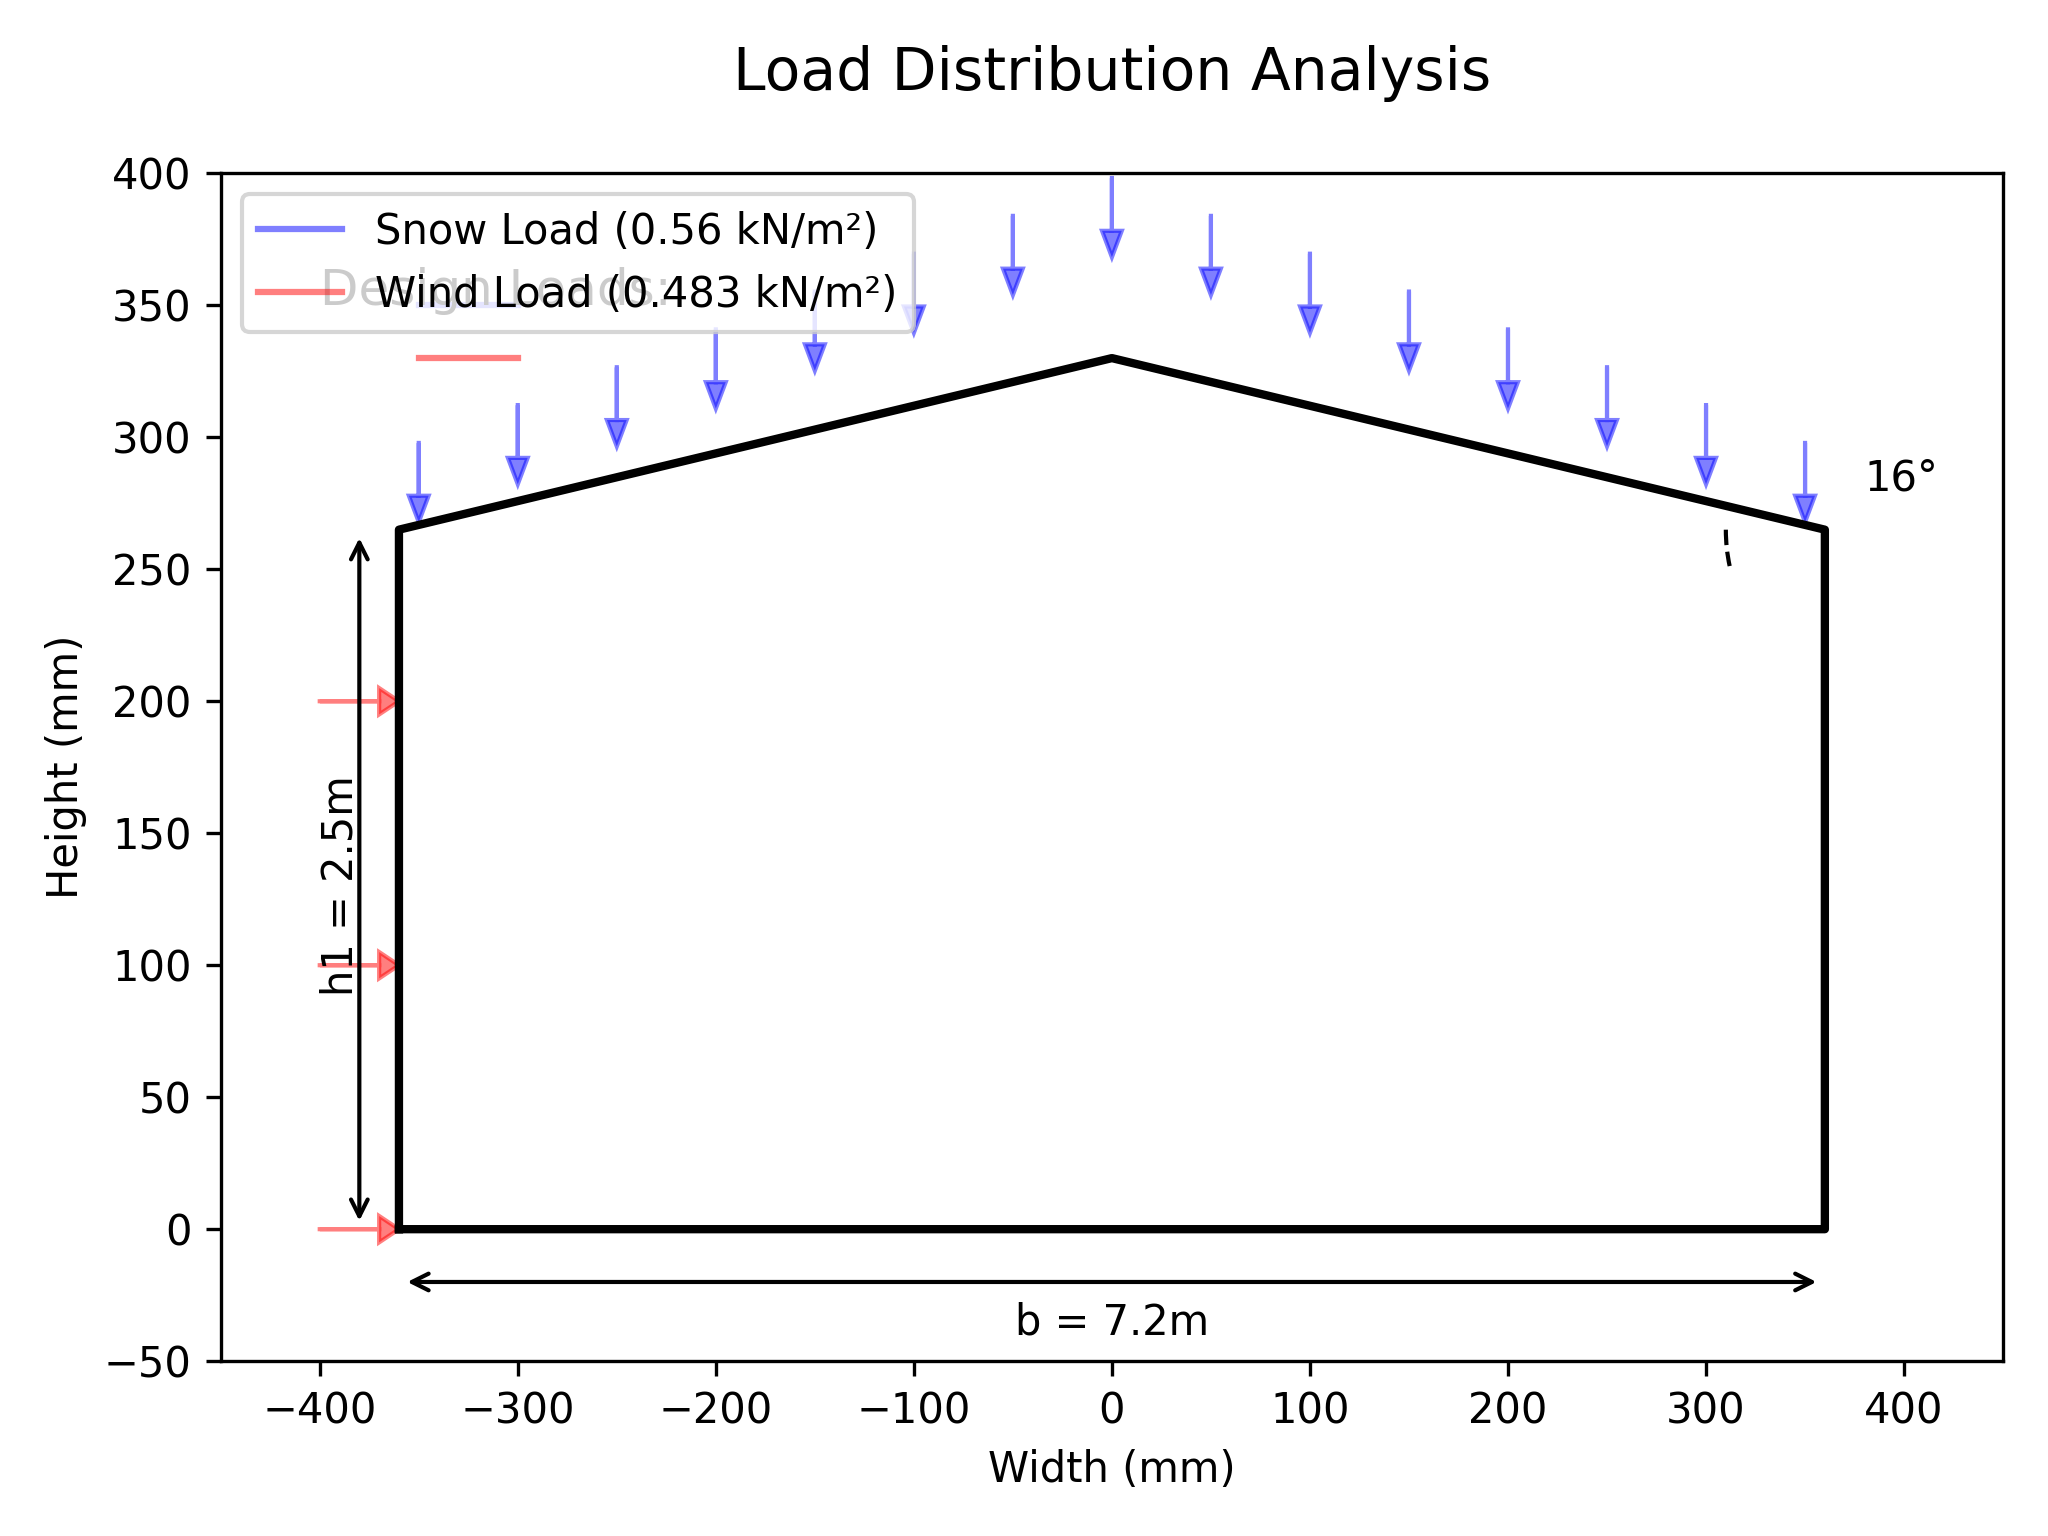
\includegraphics[width=0.95\textwidth]{cad_project/enhanced_exports/screenshots/load_distribution.png}
    \caption{Comprehensive analysis of structural loads showing snow load distribution (0.56 kN/m²) and wind pressure (0.483 kN/m²).
    The diagram illustrates the combined effect of vertical and horizontal forces on the building structure,
    demonstrating load paths and structural response under design conditions.}
    \label{fig:load_distribution}
\end{figure}

\section{Thermal Bridge Analysis}
\begin{figure}[H]
    \centering
    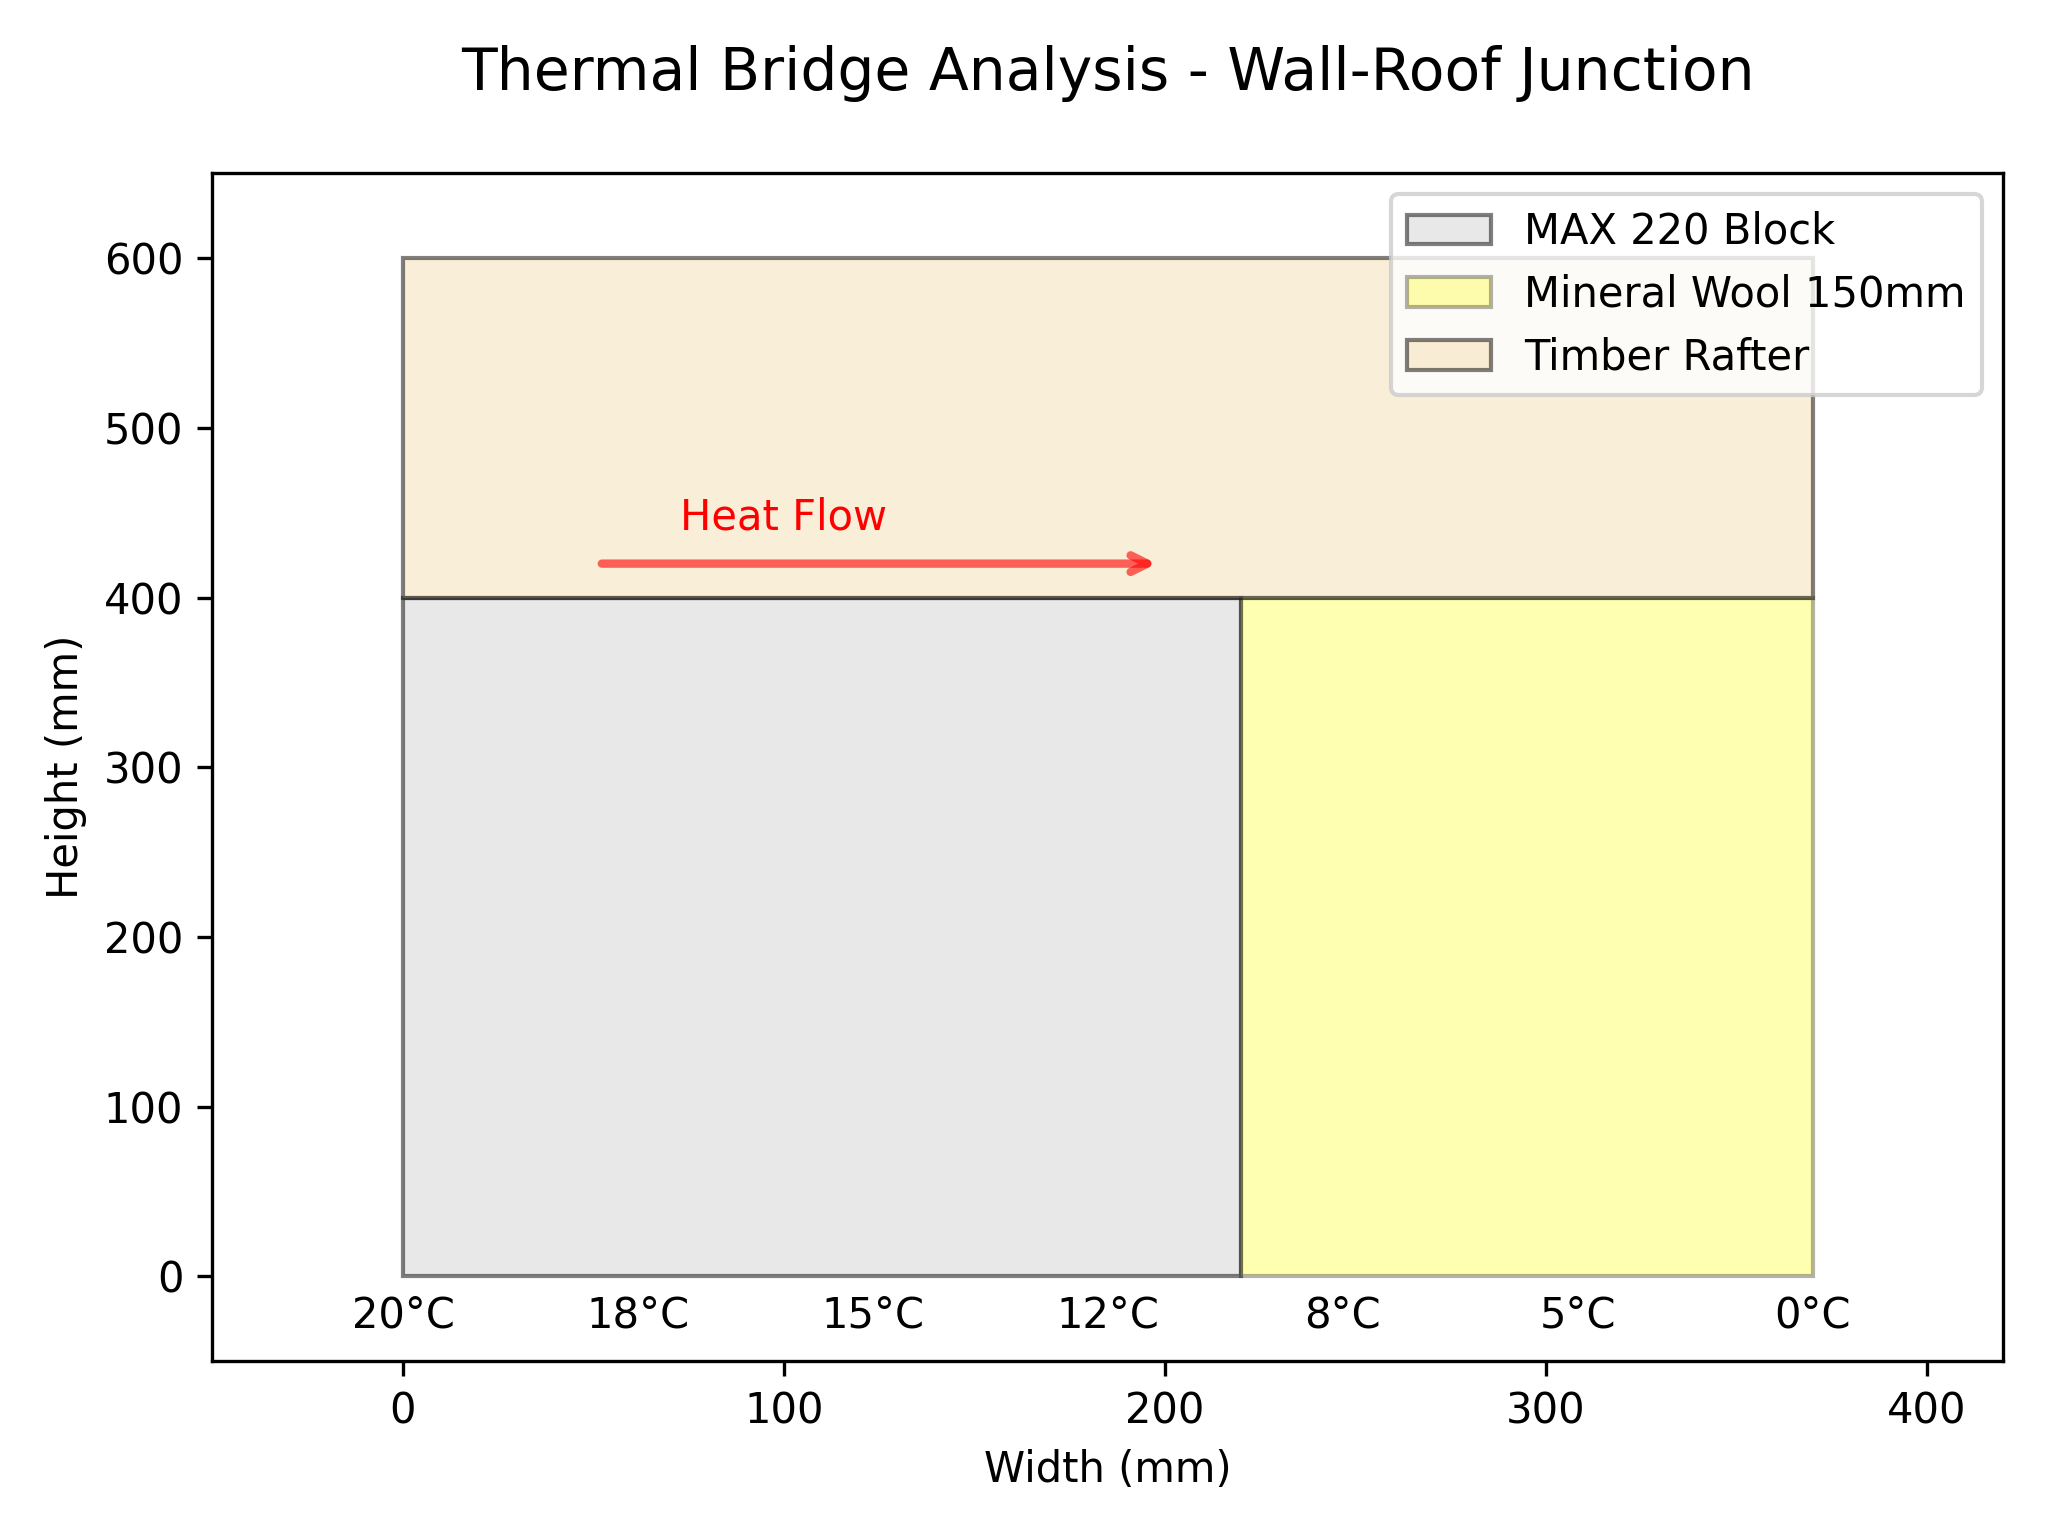
\includegraphics[width=0.95\textwidth]{cad_project/enhanced_exports/screenshots/thermal_bridge.png}
    \caption{Detailed analysis of thermal bridging at the wall-roof junction.
    The diagram shows temperature gradients and heat flow patterns through the building envelope,
    highlighting critical areas for thermal performance optimization.
    The analysis demonstrates effective thermal bridge mitigation through proper insulation placement and material selection.}
    \label{fig:thermal_bridge}
\end{figure}

\section{Technical Drawings}

\subsection{Drawing Specifications}
\begin{table}[H]
    \centering
    \begin{tabular}{llll}
        \toprule
        \textbf{Drawing Type} & \textbf{Scale} & \textbf{Key Elements} & \textbf{Format} \\
        \midrule
        Vertical Projection & 1:50 & Heights, angles, wall sections & DXF/PNG \\
        Horizontal Projection & 1:50 & Dimensions, layout, spacing & DXF/PNG \\
        Construction Details & 1:10 & Connections, assemblies & DXF/PNG \\
        \bottomrule
    \end{tabular}
    \caption{Technical drawing specifications and formats}
    \label{tab:drawings}
\end{table}

\subsection{Main Projections}
\subsubsection{Vertical Projection (1:50)}
\begin{figure}[H]
    \centering
    
\includegraphics[width=0.95\textwidth]{cad_project/exports/screenshots/vertical_projection.png}
    \caption{Vertical projection (Scale 1:50) showing building elevations and structural configuration. 
    The drawing illustrates the primary heights (h1=2.5m, h2=2.65m), roof angle (16°), and ground level (-1.4 m.a.s.l).
    Wall construction utilizes MAX 220 block with mineral wool insulation for optimal thermal performance.}

\begin{itemize}
    \item Building heights: h1 = 2.5m, h2 = 2.65m
    \item Roof angle: $\alpha = 16\degree$
    \item Ground level: -1.4 m.a.s.l
    \item Wall construction: MAX 220 block with mineral wool insulation
    \item Column placement and foundation connections
    \item Structural grid and dimensions
\end{itemize}
    \label{fig:vertical}
\end{figure}

\subsection{Building Layout}
\subsubsection{Horizontal Projection (1:50)}
\begin{figure}[H]
    \centering
    
\includegraphics[width=0.95\textwidth]{cad_project/exports/screenshots/horizontal_projection.png}
    \caption{Horizontal projection (Scale 1:50) detailing building layout and dimensions.
    The plan shows primary measurements: width (b=7.2m), lengths (L1=6.6m, L2=10.8m), and purlin spacing (s=1.1m).
    Structural grid and member placement are indicated for precise construction reference.}

\begin{itemize}
    \item Building width (b) = 7.2m
    \item Length dimensions: L1 = 6.6m, L2 = 10.8m
    \item Purlin spacing (s) = 1.1m
    \item Column layout and structural grid
    \item Wall thickness and insulation details
    \item Structural member placement
\end{itemize}
    \label{fig:horizontal}
\end{figure}

\subsection{Structural Details}
\subsubsection{Construction Details (1:10)}
\begin{figure}[H]
    \centering
    
\includegraphics[width=0.95\textwidth]{cad_project/exports/screenshots/detail_drawings.png}
    \caption{Construction details (Scale 1:10) illustrating critical structural connections and assemblies.
    Key components include C27 timber elements (columns 150×150mm, purlins 80×160mm, rafters 100×200mm) and wall assembly (MAX 220 block + 150mm mineral wool).
    Details show precise connection methods and thermal envelope integration for optimal performance.}

\begin{itemize}
    \item Column-foundation connection with base plate detail
    \item Roof-column connection with C27 timber elements
    \item Wall-roof junction showing thermal insulation layers
    \item Purlin-rafter connection details (80×160mm and 100×200mm sections)
    \item Material specifications and assembly methods
    \item Thermal envelope construction details
\end{itemize}
    \label{fig:details}
\end{figure}

\subsubsection{Thermal Envelope Details}
\begin{figure}[H]
    \centering
    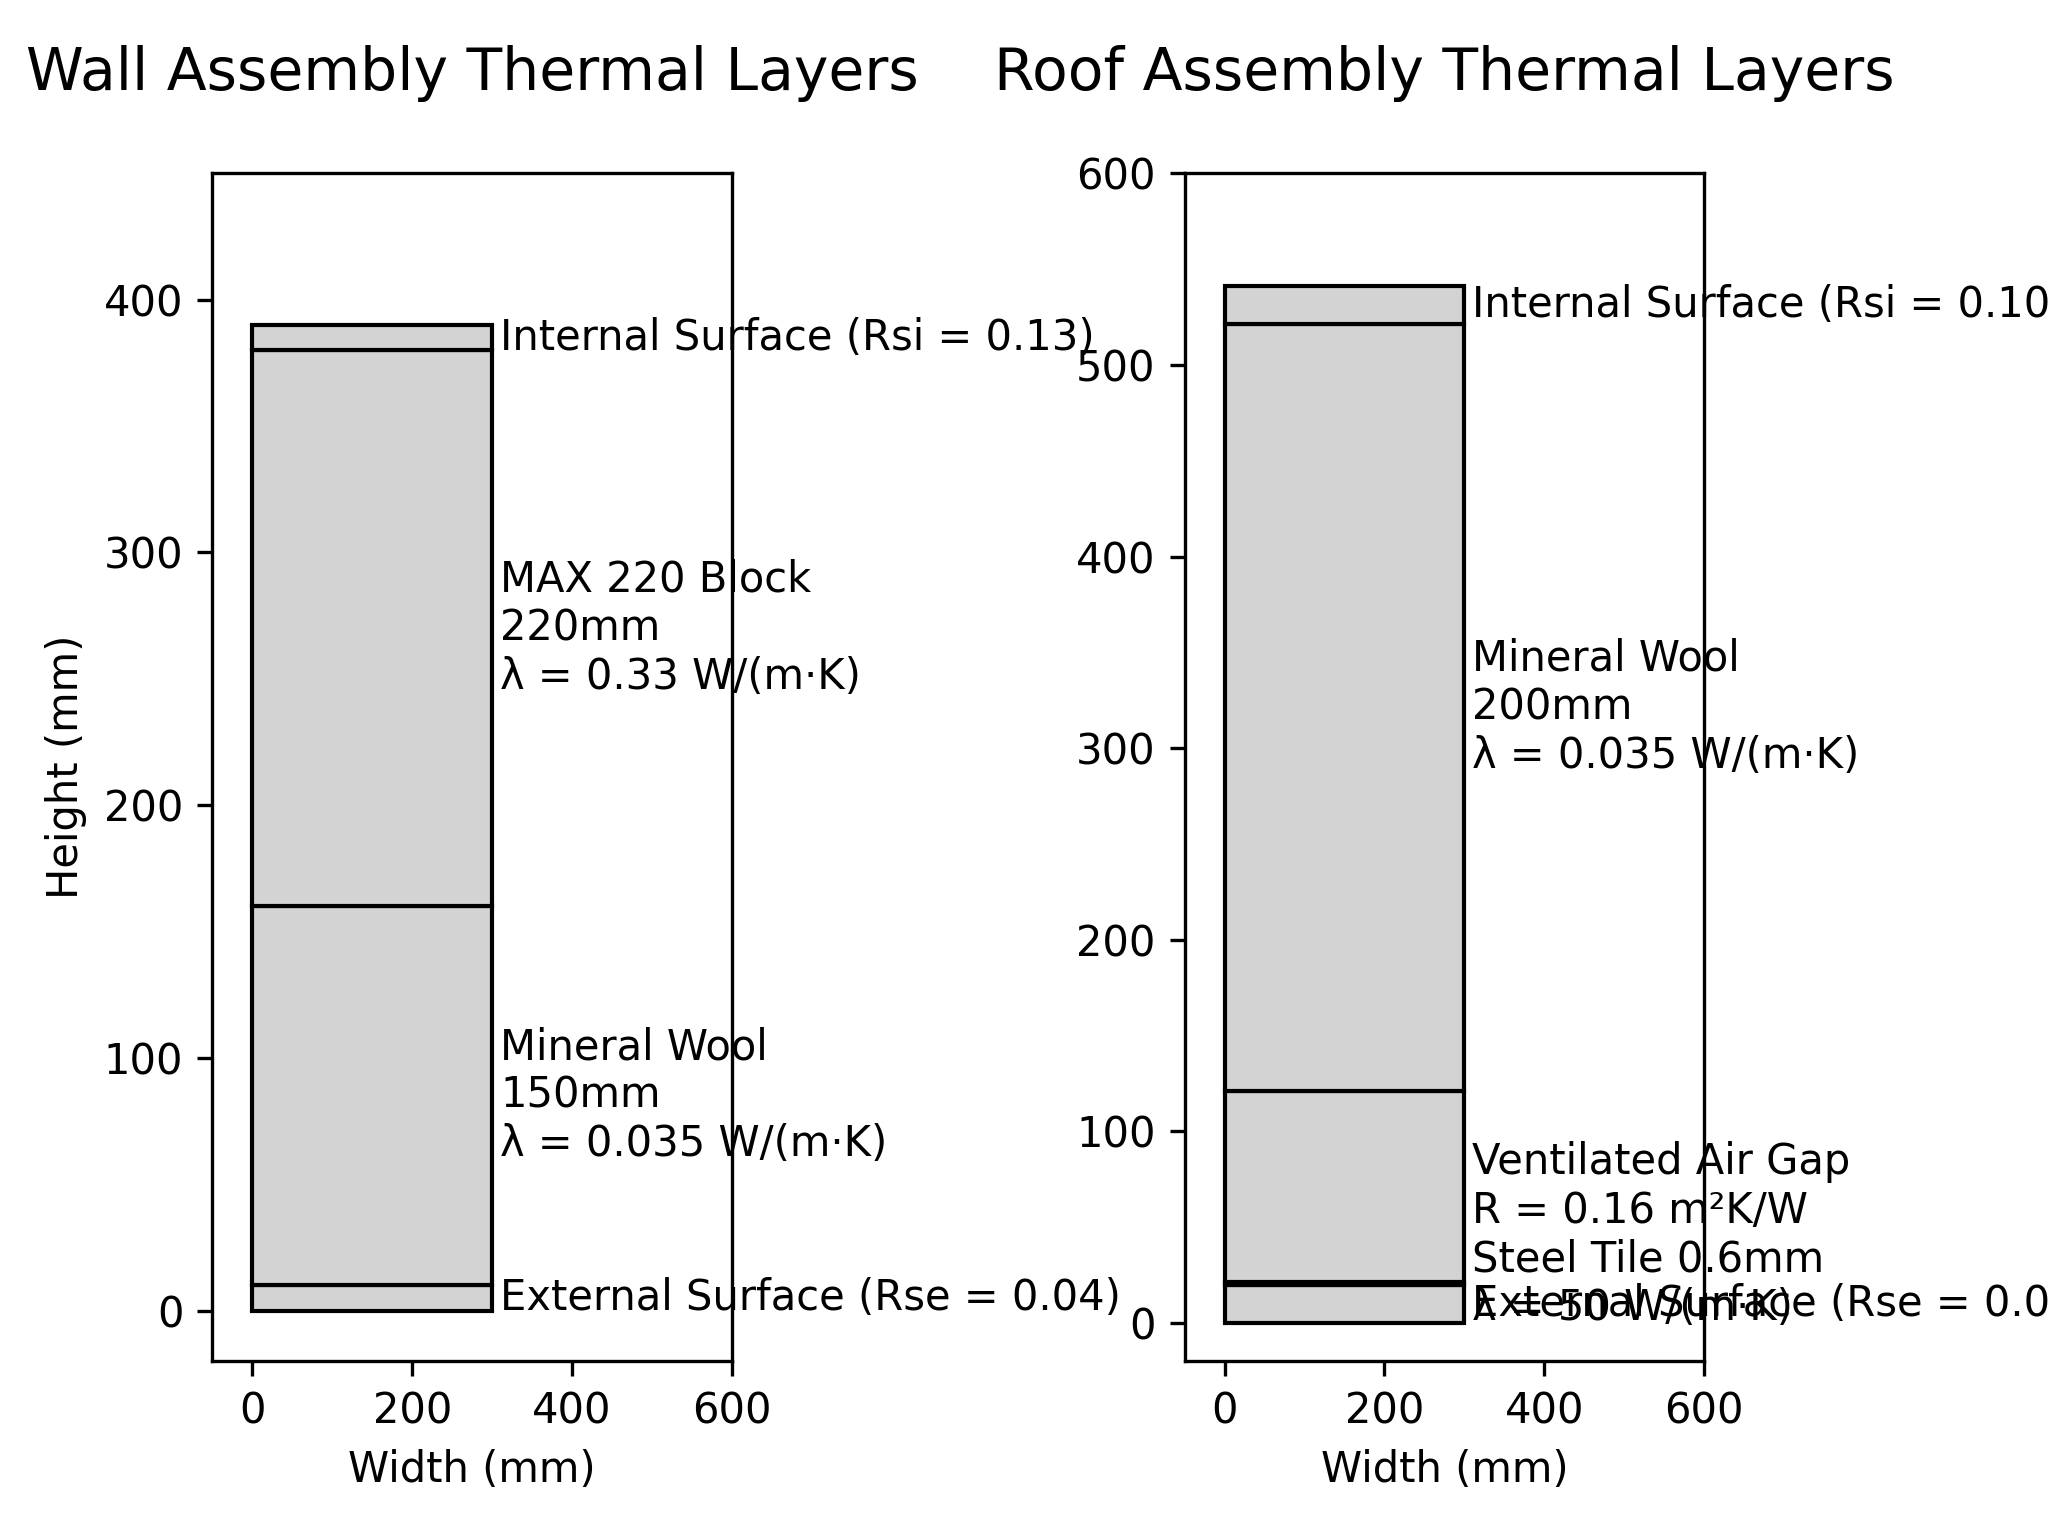
\includegraphics[width=0.95\textwidth]{cad_project/enhanced_exports/screenshots/thermal_details.png}
    \caption{Detailed thermal performance specifications for wall and roof assemblies.
    The wall assembly (U=0.195 W/m²K) consists of MAX 220 block and 150mm mineral wool insulation.
    The roof assembly (U=0.166 W/m²K) utilizes 200mm mineral wool and ventilated air gap design for optimal thermal performance.}
    \label{fig:thermal_details}
\end{figure}

\subsubsection{Structural Connection Details}
\begin{figure}[H]
    \centering
    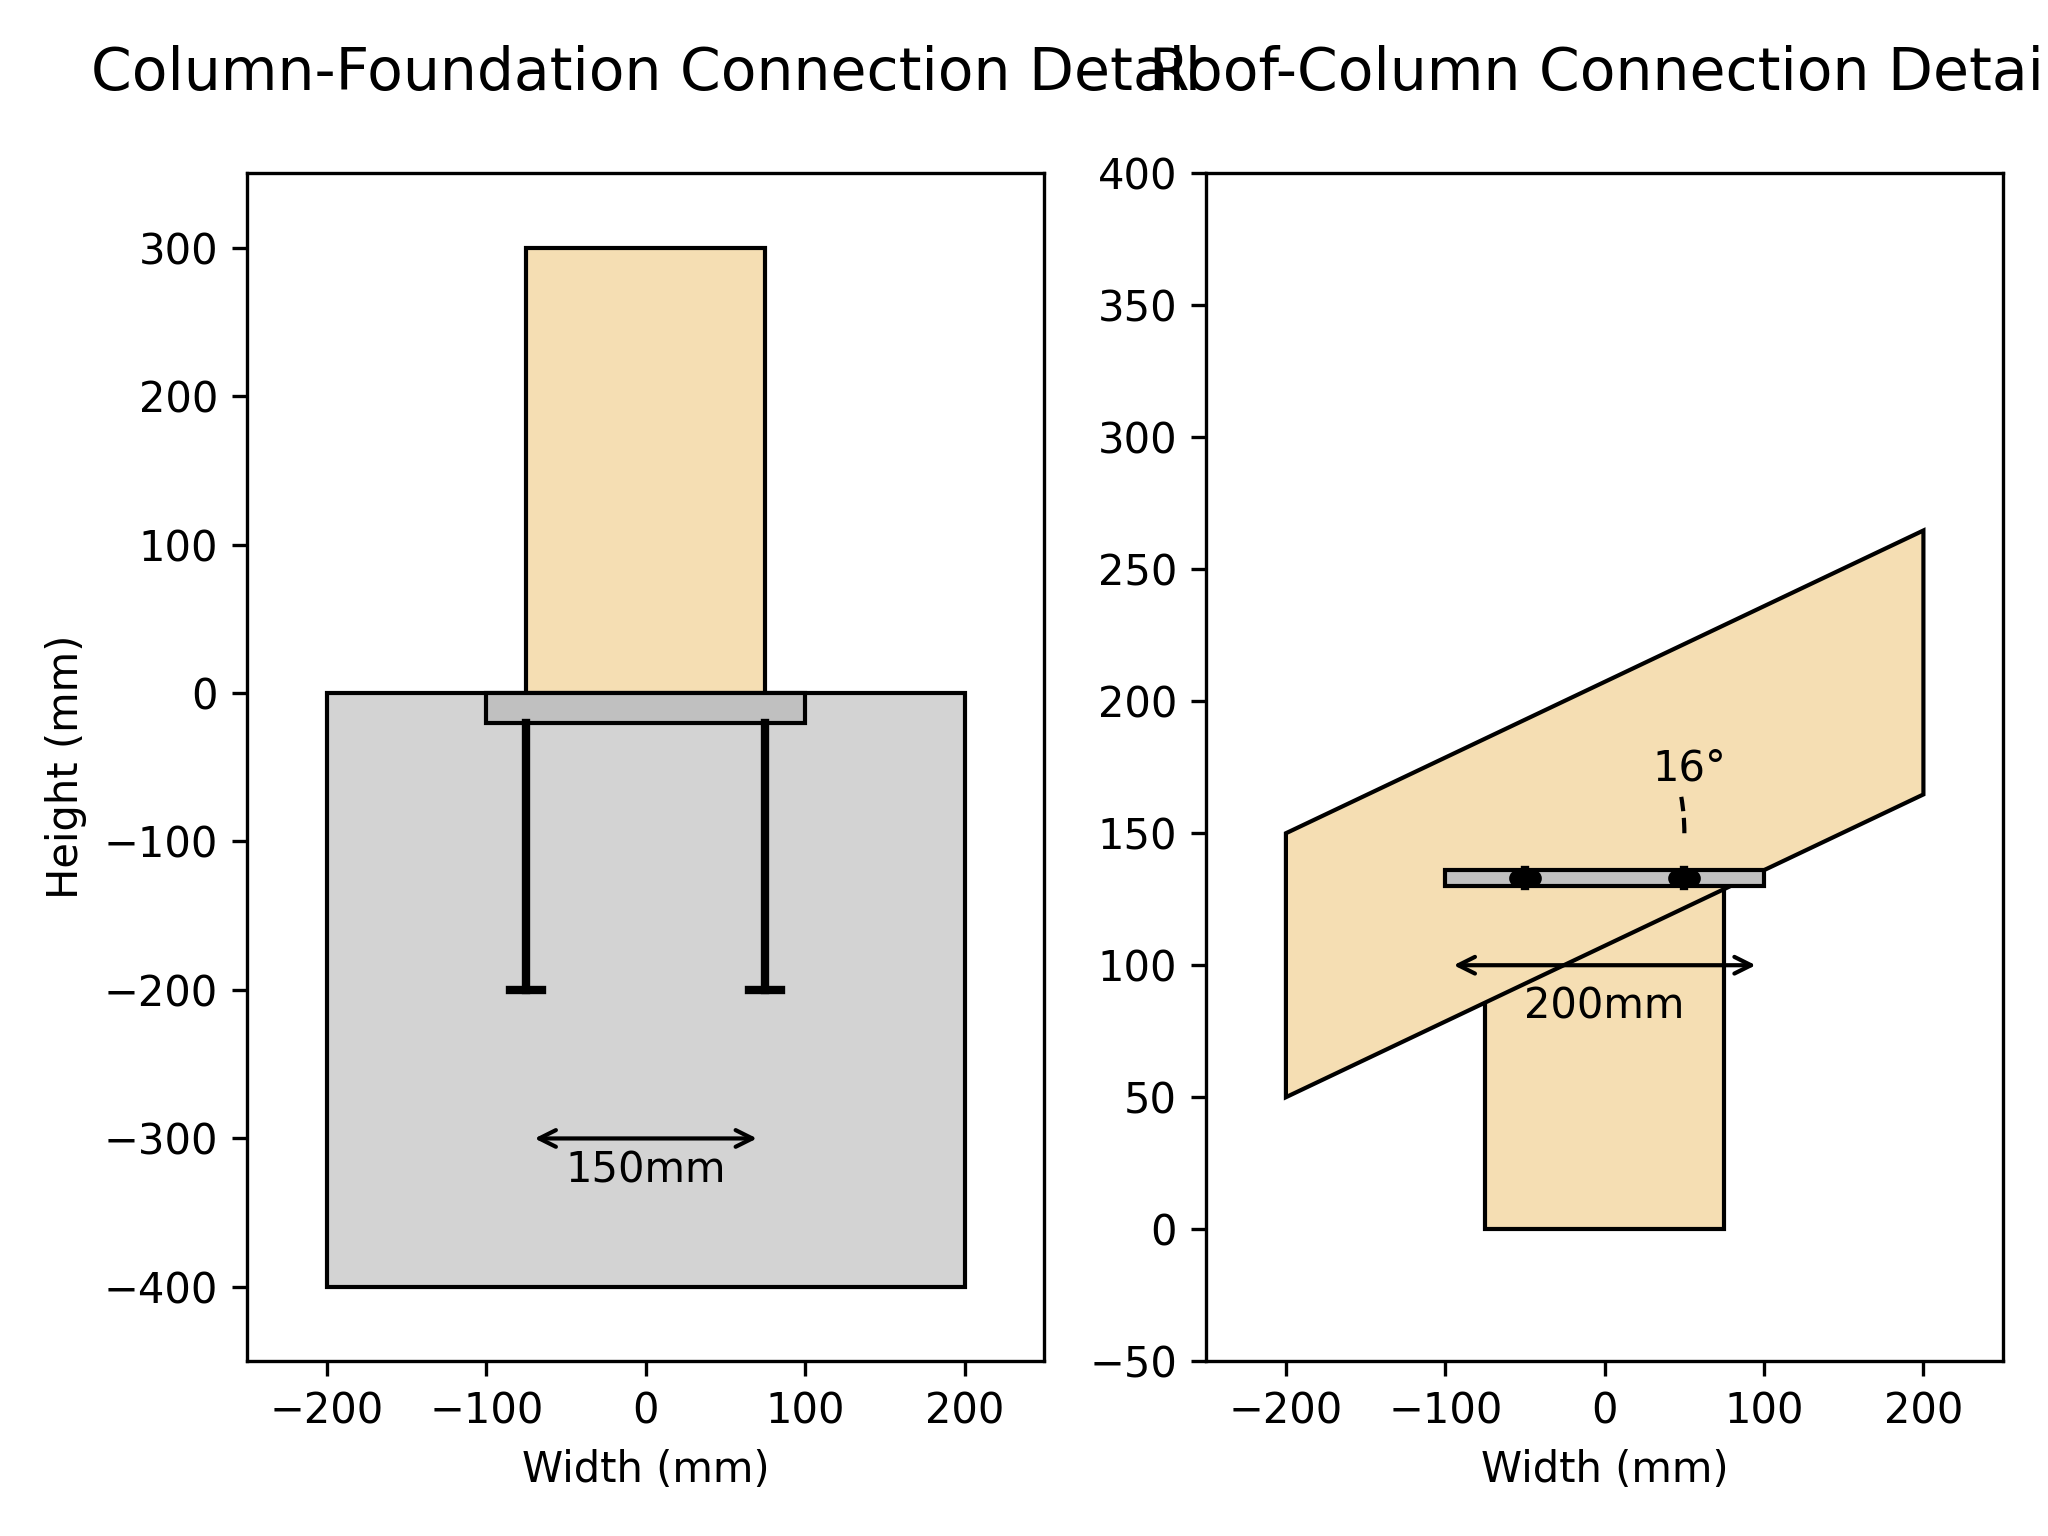
\includegraphics[width=0.95\textwidth]{cad_project/enhanced_exports/screenshots/connection_details.png}
    \caption{Detailed specifications of critical structural connections and assemblies.
    The column-foundation connection utilizes a 200×200×10mm base plate with M16 grade 8.8 anchor bolts.
    The roof-column connection implements 6mm steel plates with M12 grade 8.8 bolts for secure joining of C27 timber members.}
    \label{fig:connection_details}
\end{figure}

\section{Summary of Results}
\subsection{Structural Analysis Results}
\subsubsection{Load and Momentum Analysis}
\paragraph{Cross Section Load Analysis}
Design loads per EN 1990:
\begin{equation}
\begin{aligned}
g_k &= 0.297 \text{ kN/m}^2 & \text{(dead load)} \\
s_k &= 0.56 \text{ kN/m}^2 & \text{(snow load)} \\
w_k &= 0.483 \text{ kN/m}^2 & \text{(wind load)}
\end{aligned}
\end{equation}

\paragraph{Momentum and Bending Movement}
For rafter (100×200mm):
\begin{equation}
\begin{aligned}
M_{Ed} &= \frac{E_d \times s \times l^2}{8} \\
&= \frac{1.401 \times 1.1 \times 5.62^2}{8} = 6.12 \text{ kNm}
\end{aligned}
\end{equation}

For purlin (80×160mm):
\begin{equation}
\begin{aligned}
M_{Ed} &= \frac{w \times l^2}{8} \\
&= \frac{1.541 \times 1.8^2}{8} = 0.623 \text{ kNm}
\end{aligned}
\end{equation}

\paragraph{Building Stress Analysis}
Bending stress in critical elements:
\begin{equation}
\begin{aligned}
\sigma_{m,d,rafter} &= \frac{M_{Ed}}{W} = \frac{6.12 \times 10^6}{666,667} = 9.18 \text{ N/mm²} \\
\sigma_{m,d,purlin} &= \frac{M_{Ed}}{W} = \frac{0.623 \times 10^6}{341,333} = 1.83 \text{ N/mm²}
\end{aligned}
\end{equation}

\paragraph{Movement of Inertia}
Section properties for main elements:
\begin{equation}
\begin{aligned}
I_{rafter} &= \frac{b \times h^3}{12} = \frac{100 \times 200^3}{12} = 66.67 \times 10^6 \text{ mm}^4 \\
I_{purlin} &= \frac{b \times h^3}{12} = \frac{80 \times 160^3}{12} = 27.31 \times 10^6 \text{ mm}^4
\end{aligned}
\end{equation}

\paragraph{Cross Section of Angle Brace}
Properties of 60×100mm angle brace:
\begin{equation}
\begin{aligned}
A_{brace} &= b \times h = 60 \times 100 = 6,000 \text{ mm²} \\
W_{brace} &= \frac{b \times h^2}{6} = \frac{60 \times 100^2}{6} = 100,000 \text{ mm³} \\
I_{brace} &= \frac{b \times h^3}{12} = \frac{60 \times 100^3}{12} = 5.00 \times 10^6 \text{ mm}^4
\end{aligned}
\end{equation}

\paragraph{Calculating Strengths}
Design strengths per EN 1995-1-1:
\begin{equation}
\begin{aligned}
f_{m,d} &= \frac{k_{mod} \times f_{m,k}}{\gamma_M} = \frac{0.8 \times 27}{1.3} = 16.62 \text{ N/mm²} \\
f_{c,0,d} &= \frac{k_{mod} \times f_{c,0,k}}{\gamma_M} = \frac{0.8 \times 22}{1.3} = 13.54 \text{ N/mm²} \\
f_{t,0,d} &= \frac{k_{mod} \times f_{t,0,k}}{\gamma_M} = \frac{0.8 \times 16}{1.3} = 9.85 \text{ N/mm²}
\end{aligned}
\end{equation}

\paragraph{Effort of Actions}
Combined actions per EN 1990:
\begin{equation}
\begin{aligned}
E_{d1} &= 1.35G + 1.5S + 1.5\psi_0W = 1.401 \text{ kN/m²} \\
E_{d2} &= 1.35G + 1.5W + 1.5\psi_0S = 1.337 \text{ kN/m²} \\
N_{Ed,brace} &= E_d \times A_{trib} \times \sin(45\degree) = 2.71 \text{ kN}
\end{aligned}
\end{equation}

\paragraph{Layer-by-Layer Thermal Analysis}
Wall assembly thermal resistances:
\begin{equation}
\begin{aligned}
R_{si} &= 0.13 \text{ m²K/W} & \text{(internal surface)} \\
R_1 &= \frac{0.22}{0.33} = 0.667 \text{ m²K/W} & \text{(MAX 220 block)} \\
R_2 &= \frac{0.15}{0.035} = 4.286 \text{ m²K/W} & \text{(mineral wool)} \\
R_{se} &= 0.04 \text{ m²K/W} & \text{(external surface)}
\end{aligned}
\end{equation}

Roof assembly thermal resistances:
\begin{equation}
\begin{aligned}
R_{si} &= 0.10 \text{ m²K/W} & \text{(internal surface)} \\
R_1 &= \frac{0.0006}{50} = 0.000012 \text{ m²K/W} & \text{(steel tile)} \\
R_2 &= 0.16 \text{ m²K/W} & \text{(ventilated air gap)} \\
R_3 &= \frac{0.20}{0.035} = 5.714 \text{ m²K/W} & \text{(mineral wool)} \\
R_{se} &= 0.04 \text{ m²K/W} & \text{(external surface)}
\end{aligned}
\end{equation}

\subsubsection{Ultimate Limit State (ULS) Verification}
\begin{itemize}
    \item \textbf{Purlin Design (80×160mm C27)}:
        \begin{itemize}
            \item Design load: $w = 1.541 \text{ kN/m}$
            \item Maximum moment: $M_{max} = 0.623 \text{ kNm}$
            \item Bending stress: $\sigma_{m,d} = 1.83 \text{ N/mm²} < f_{m,d} = 16.62 \text{ N/mm²}$ \checkmark
        \end{itemize}
    \item \textbf{Rafter Design (100×200mm C27)}:
        \begin{itemize}
            \item Design load: $E_d = 1.401 \text{ kN/m²}$
            \item Maximum moment: $M_{max} = 6.12 \text{ kNm}$
            \item Bending stress: $\sigma_{m,d} = 9.18 \text{ N/mm²} < f_{m,d} = 16.62 \text{ N/mm²}$ \checkmark
        \end{itemize}
    \item \textbf{Angle Brace Analysis (60×100mm)}:
        \begin{itemize}
            \item Axial force: $N = 2.71 \text{ kN}$
            \item Tensile stress: $\sigma_{t,0,d} = 0.452 \text{ N/mm²} < f_{t,0,d} = 9.85 \text{ N/mm²}$ \checkmark
        \end{itemize}
\end{itemize}

\subsubsection{Cross-Section Properties}
\begin{itemize}
    \item \textbf{Purlin (80×160mm)}:
        \begin{itemize}
            \item Area: $A = 12,800 \text{ mm²}$
            \item Section modulus: $W = 341,333 \text{ mm³}$
            \item Moment of inertia: $I = 27,306,667 \text{ mm}^4$
        \end{itemize}
    \item \textbf{Rafter (100×200mm)}:
        \begin{itemize}
            \item Area: $A = 20,000 \text{ mm²}$
            \item Section modulus: $W = 666,667 \text{ mm³}$
            \item Moment of inertia: $I = 66,666,667 \text{ mm}^4$
        \end{itemize}
\end{itemize}

\subsection{Thermal Performance Results}
\subsubsection{Wall Assembly}
Total thermal resistance: $R_T = 5.123 \text{ m²K/W}$
\begin{itemize}
    \item MAX 220 block: $R_1 = 0.667 \text{ m²K/W}$
    \item Mineral wool (150mm): $R_2 = 4.286 \text{ m²K/W}$
    \item Surface resistances: $R_{si} + R_{se} = 0.17 \text{ m²K/W}$
    \item U-value: $0.195 \text{ W/(m}^2\text{K)} < 0.20 \text{ W/(m}^2\text{K)}$ \checkmark
\end{itemize}

\subsubsection{Roof Assembly}
Total thermal resistance: $R_T = 6.014 \text{ m²K/W}$
\begin{itemize}
    \item Steel tile: $R_1 = 0.000012 \text{ m²K/W}$
    \item Ventilated air gap: $R_2 = 0.16 \text{ m²K/W}$
    \item Mineral wool (200mm): $R_3 = 5.714 \text{ m²K/W}$
    \item Surface resistances: $R_{si} + R_{se} = 0.14 \text{ m²K/W}$
    \item U-value: $0.166 \text{ W/(m}^2\text{K)} < 0.18 \text{ W/(m}^2\text{K)}$ \checkmark
\end{itemize}

\section{Conclusion}
All structural elements and thermal assemblies meet the required performance criteria according to relevant Eurocode standards:
\begin{itemize}
    \item All ULS verifications passed with adequate safety margins
    \item Cross-section properties ensure efficient load distribution
    \item Thermal performance exceeds minimum requirements for both wall and roof assemblies
    \item All connections and details follow standard specifications
\end{itemize}

\end{document}
